\documentclass[pdftex,12pt,a4paper]{report}

\usepackage[portuguese,english]{babel}
\usepackage[T1]{fontenc} 
\usepackage[table]{xcolor}
\usepackage[utf8]{inputenc}
\usepackage[pdftex]{graphicx}
\usepackage{minitoc}
\usepackage{hyperref}
\usepackage{indentfirst}
\usepackage[compact]{titlesec}
\usepackage{fancyhdr}
\usepackage{caption}
\usepackage{pgfplots}
\usepackage{pgfplotstable}
\usepackage{fixltx2e}
\usepackage{mathtools}
\usepackage{fancyhdr}
\usepackage{listings}
\usepackage{color}
\usepackage{sverb}
\usepackage[section]{placeins}
%Highlight
\newcommand{\shellcmd}[1]{\\\indent\indent\texttt{\footnotesize\# #1}\\}

\pagestyle{fancy}
\renewcommand*\thesection{\thechapter\arabic{section}}
\newcommand{\HRule}{\rule{\linewidth}{0.5mm}}
\begin{document}

\begin{titlepage}

\begin{center}


\includegraphics[width=0.15\textwidth]{./logo}\\[0.5cm]    

\textsc{\large Universidade de Aveiro \\[1cm]\large departamento de electrónica, telecomunicações e informática}\\[1cm]

\textsc{\large{47022}\large - Arquitectura de Computadores Avançada \\[1cm]}

\HRule \\[0.5cm]
{ \huge \bfseries  Home group assignment 1}\\[0.4cm]
{ \large \bfseries Implementing a forwarding and stall unit in a pipelined architecture}\\[0.4cm]
\HRule \\[1cm]

\textsc{\small{8240 - MESTRADO INTEGRADO EM ENGENHARIA DE COMPUTADORES E TELEMÁTICA}}\\[1cm]

\begin{minipage}{0.4\textwidth}

\begin{flushleft} \large
\href{mailto:rafael.ferreira@ua.pt}{António Rafael da \\ Costa Ferreira }
 \small{\\NMec: 67405 | P4G1}
\end{flushleft}
\end{minipage}
\begin{minipage}{0.4\textwidth}

\begin{flushright} \large
\href{mailto:rodrigocunha@ua.pt}{Rodrigo Lopes \\ da Cunha}
\small{\\NMec: 67800 | P4G1}
\end{flushright}
\end{minipage}\\[1cm]

{\large Docentes: Nuno Lau/José Luís Azevedo   }\\[0.5cm]

\vfill

{\large Novembro de 2015 \\ 2015-2016}

\end{center}

\end{titlepage} %Titulo do Relatorio
\renewcommand{\headrulewidth}{0pt}

%Cabeçalhos de rodapé
\fancyhead{}
\fancyfoot{}
\lhead{Home group assignment 2}
\rhead{ACA - 2015/2016}
\lfoot{Rafael Ferreira nmec: 67405 \\ Rodrigo Cunha nmec: 67800}
\rfoot{\thepage}

%Renomear Comandos
\renewcommand*\contentsname{Conteúdos}
\renewcommand*\figurename{Figura}
\renewcommand*\tablename{Tabela}

%Conteúdos, dar paragrafo
\tableofcontents
%Headers
\renewcommand{\headrulewidth}{0.15pt}
\renewcommand{\thechapter}{}

\clearpage

\section{Introdução}
% o que, porquê e o objetivo

O trabalho proposto para a unidade curricular de Arquitetura de Computadores Avançada foi a implementação em CUDA para o processamento de um Semi-Global Matching. 

Este programa tem como objetivo determinar a imagem de disparidade entre duas imagens idênticas mas de posições diferentes, como se de dois olhos se tratasse, uma vista com o olho da esquerda e outra com o olho da direita.

O relatório reflete todas as geometrias de kernel implementadas, formas de pensamento, métodos de como foram implementados os algoritmos, resultados, tutorial para correr o código elaborado, e por último a conclusão deste mesmo trabalho.

\newpage
\section{Exercício 1}

\subsection{Cuda Kernel da função "determine\_costs()"}
Neste primeiro exercício, era pedido que se desenvolvesse um kernel em CUDA que substituísse a função \textit{determine\_costs()}.

\begin{figure}[!htb]
\center
 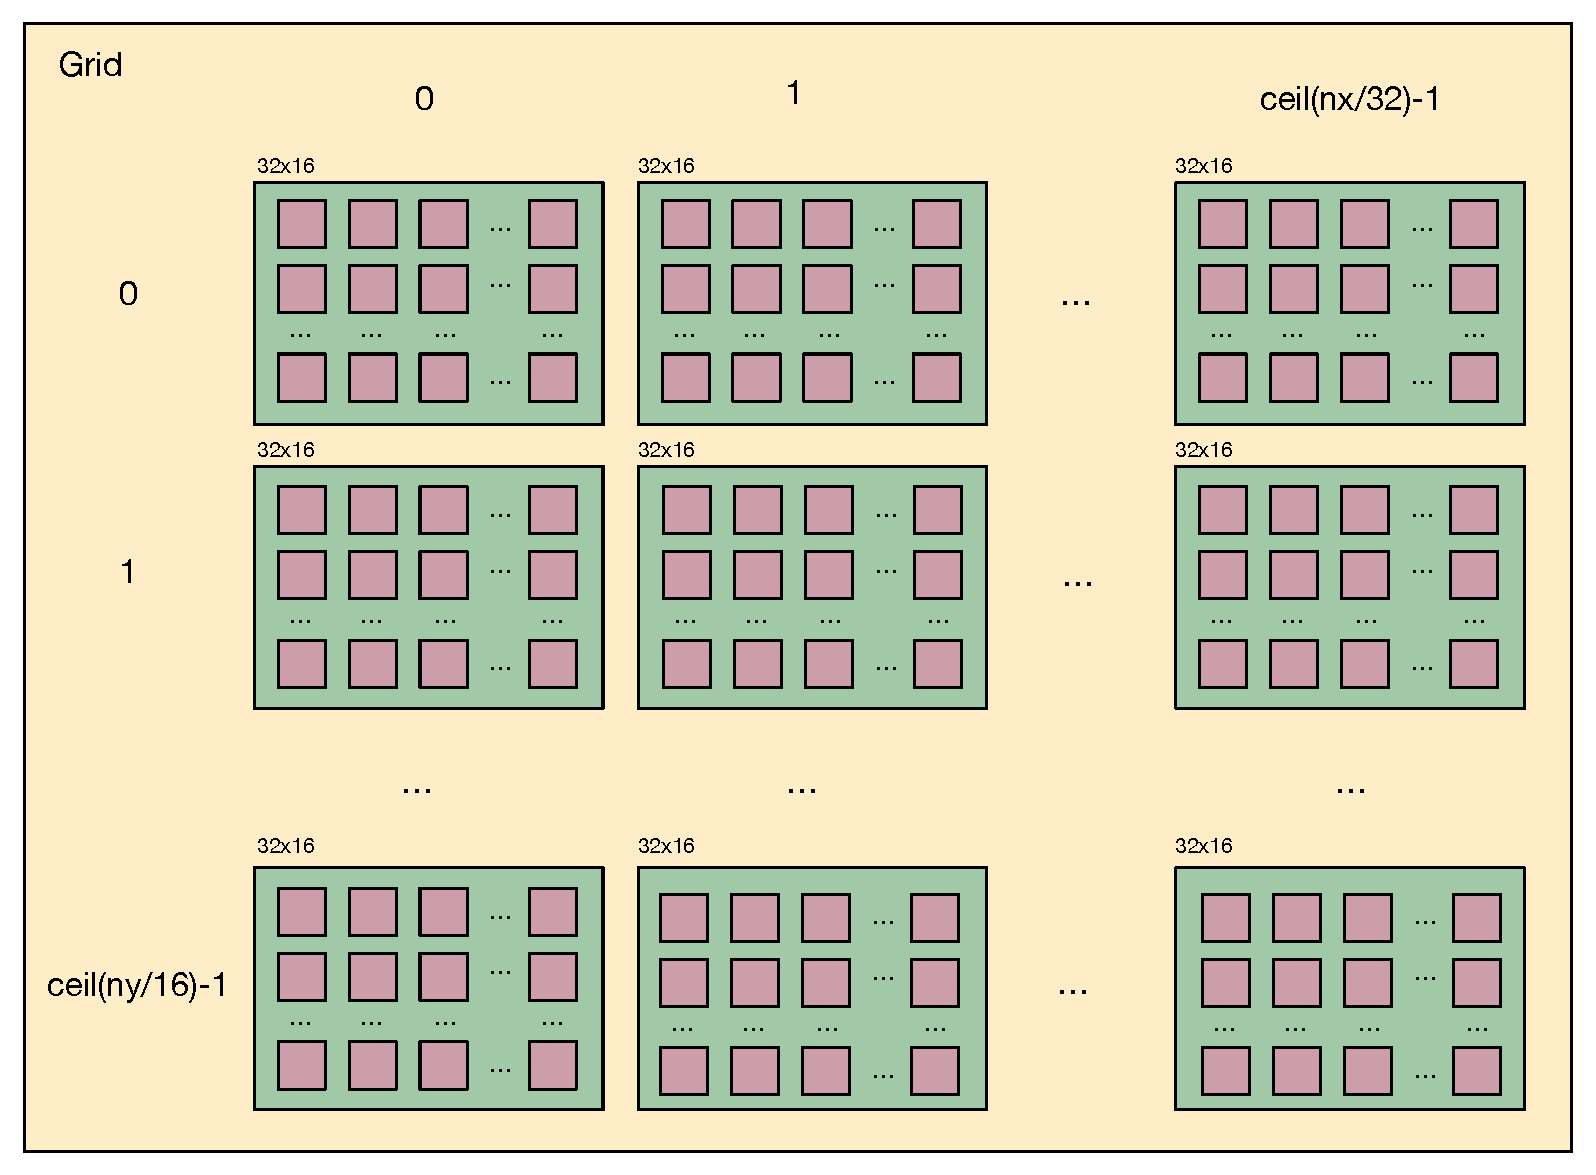
\includegraphics[width=100mm,scale=1]{DetermineCosts_v1_kernel.pdf}
 \caption{\\ Geometria do Kernel para a função determine\_costs()}
 \label{fig:DetermineCosts_v1_kernel}
\end{figure}

Neste kernel optou-se por uma geometria (Figura \ref{fig:DetermineCosts_v1_kernel}  constituída por uma grid de tamanho (ceil(nx\/32) x ceil(ny\/16)) com blocos de 32 x 16 threads cada.
Nesta função, cada thread corresponde a um pixel da imagem, e cada um calcula o valor de custo, sendo este a diferença entre as imagens num determinado pixel.

Este exercicío foi ainda realizado de duas maneira, uma utilizando a \textit{global memory}, e outra onde se coloca as imagens e o valor de COSTS na \textit{texture memory}. 

Para a \textit{global memory} utilizou-se o seguinte algoritmo para desenvolver o kernel:

\begin{lstlisting}[language=c++, basicstyle=\scriptsize]
__global__ void determine_costs_device(const int *left_image,  const int *right_image,
 int *costs, 
const int nx, const int ny, const int disp_range)
{
  int i = blockIdx.x * blockDim.x + threadIdx.x;
  int j = blockIdx.y * blockDim.y + threadIdx.y;

  if (i < nx && j < ny)
  {
    for ( int d = 0; d < disp_range; d++ ) {
      if(i >= d){
        COSTS(i,j,d) = abs( LEFT_IMAGE(i,j) - RIGHT_IMAGE(i-d,j));
      }
    }
  }
}
\end{lstlisting} 

Com esta implementação obtiveram-se os seguintes resultados:

\begin{figure}[!htb]
\center
 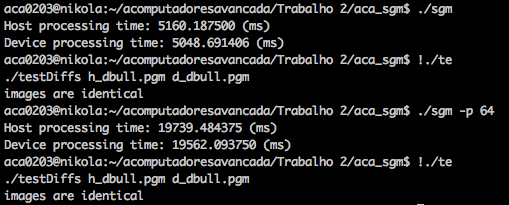
\includegraphics[width=100mm,scale=1]{DetermineCostsv1globalresults.png}
 \caption{\\ Resultados obtidos utilizando global memory}
 \label{fig:DetermineCostsv1globalresults}
\end{figure}


TEXTURE MEMORY CODIGO E RESULTADOS

\newpage
\section{Exercício 2}

\subsection{Cuda Kernel(s) da função "iterate\_direction\_dirxpos\_dev()" e das funções correspondestes a outras direcções}

Para este exercicío foram implementadas duas versões para a utilização de \textit{global memory}, sendo a versão 2 (otimizada) utilizada na utilização da \textit{shared memory}.

\subsubsection{Global Memory - Versão 1}

Nesta versão, foram criadas duas geometrias apenas, sendo que uma diz respeito às iterações nas direções em x, e outra em y, visto que tanto para o lado positivo como para o negativo a geometria era idêntica.

 \begin{figure}[!htb]
\center
 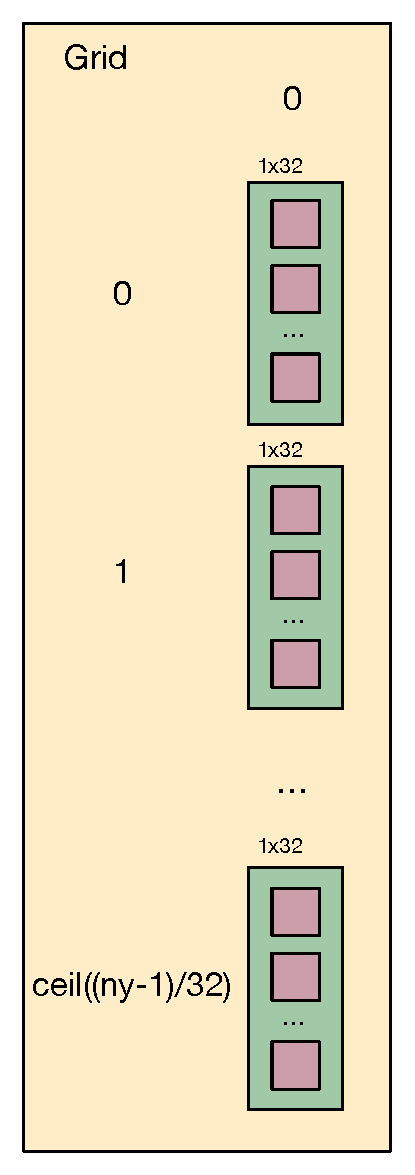
\includegraphics[width=50mm,height=100mm,scale=1]{IteratePositionDirxposneg_v1_kernel.pdf}
 \caption{\\ Geometria do Kernel para as funções iterate\_direction\_dirxpos() e iterate\_direction\_dirxneg()}
 \label{fig:IteratePositionDirxposneg_v1_kernel}
\end{figure}

Como podemos ver na figura \ref{fig:IteratePositionDirxposneg_v1_kernel}, a grid é composta por ceil(ny/32) blocos, cada bloco composto por 32 threads, sendo cada uma responsável pela linha em x onde está inserida para cálculo dos respetivos paths.

Esta operação tem de ser efetuada sequencialmente pois o pixel seguinte depende sempre do anterior, pelo que se recorreu à seguinte implementação para o kernel \textit{iterate\_direction\_dirxpos()} e para o kernel \textit{iterate\_direction\_dirxneg()}:

\begin{lstlisting}[language=c++, basicstyle=\scriptsize]
__global__ void iterate_direction_dirxpos_dev(const int dirx, const int *left_image,
                        const int* costs, int *accumulated_costs,
                        const int nx, const int ny, const int disp_range ){

      int i = 0;
      int j = blockIdx.y * blockDim.y + threadIdx.y;
      if(j < ny){

        for ( int d = 0; d < disp_range; d++ ) {
          ACCUMULATED_COSTS(0,j,d) += COSTS(0,j,d);
        }

        for(i = 1; i<nx; i++){
          evaluate_path_dev( &ACCUMULATED_COSTS(i-dirx,j,0),
                           &COSTS(i,j,0),
                           abs(LEFT_IMAGE(i,j)-LEFT_IMAGE(i-dirx,j)) ,
                           &ACCUMULATED_COSTS(i,j,0), nx, ny, disp_range);
        }
      }
}

__global__ void iterate_direction_dirxneg_dev(const int dirx, const int *left_image,
                        const int* costs, int *accumulated_costs,
                        const int nx, const int ny, const int disp_range )
{
      int i = nx-1;
      int j = blockIdx.y * blockDim.y + threadIdx.y;

      if(j < ny){

        for ( int d = 0; d < disp_range; d++ ) {
            ACCUMULATED_COSTS(nx-1,j,d) += COSTS(nx-1,j,d);
        }

        for(i = nx-2; i >= 0; i--){
            evaluate_path_dev( &ACCUMULATED_COSTS(i-dirx,j,0),
                           &COSTS(i,j,0),
                           abs(LEFT_IMAGE(i,j)-LEFT_IMAGE(i-dirx,j)),
                           &ACCUMULATED_COSTS(i,j,0), nx, ny, disp_range );
        }
      }
}
\end{lstlisting} 
\newpage
No caso da direção ser em y, então seguiu-se o mesmo pensamento que em x, obtendo a seguinte geometria:

\begin{figure}[!htb]
\center
 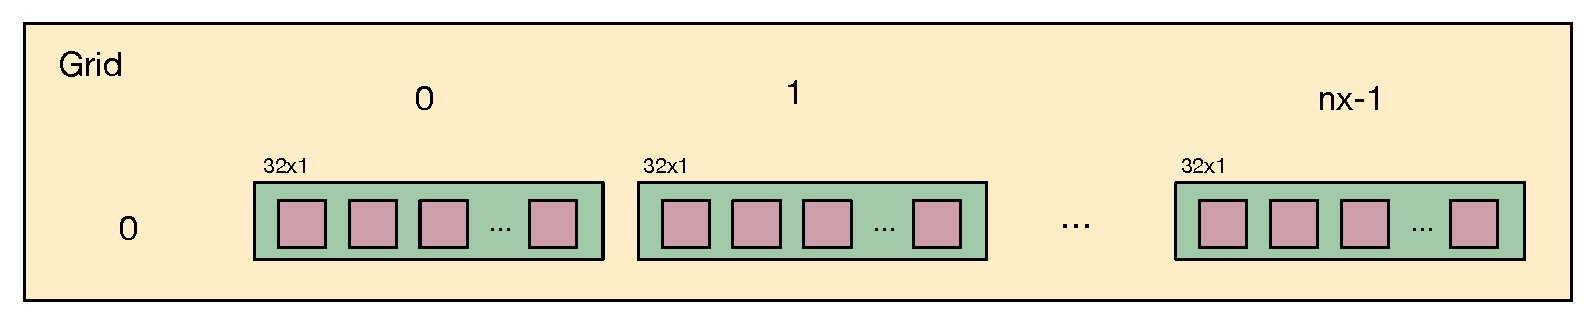
\includegraphics[width=100mm,scale=1]{IteratePositionDiryposneg_v1_kernel.pdf}
 \caption{\\ Geometria do Kernel para as funções iterate\_direction\_dirypos() e iterate\_direction\_diryneg()}
 \label{fig:IteratePositionDiryposneg_v1_kernel}
\end{figure}

Tal como apresentado na figura, neste caso a geometria é composta por uma grid de tamanho ceil(ny/32) blocos, cada um composto por 32 threads, onde cada uma volta a ser responsável pelo cálculo do respetivo caminho de todos os pixeis daquela coluna. 

Esta geometria volta a aplicar-se às direções positivas e negativa da mesma maneira tal como em x.

Foi então desenvolvido o seguinte código para os kernels \textit{iterate\_direction\_dirypos()} e \textit{iterate\_direction\_diryneg()}:

\begin{lstlisting}[language=c++, basicstyle=\scriptsize]
__global__ void iterate_direction_dirypos_dev(const int diry, const int *left_image,
                        const int* costs, int *accumulated_costs,
                        const int nx, const int ny, const int disp_range )
{
    int i = blockIdx.x * blockDim.x + threadIdx.x;
    int j = 0;
    if(i < nx){
        for ( int d = 0; d < disp_range; d++ ) {
            ACCUMULATED_COSTS(i,0,d) += COSTS(i,0,d);
        }
        for(j = 1; j<ny; j++){

          evaluate_path_dev( &ACCUMULATED_COSTS(i,j-diry,0),
                         &COSTS(i,j,0),
                         abs(LEFT_IMAGE(i,j)-LEFT_IMAGE(i,j-diry)),
                         &ACCUMULATED_COSTS(i,j,0), nx, ny, disp_range );
      }
    }
}

__global__ void iterate_direction_diryneg_dev(const int diry, const int *left_image,
                        const int* costs, int *accumulated_costs,
                        const int nx, const int ny, const int disp_range )
{

      int i = blockIdx.x * blockDim.x + threadIdx.x;
      int j = ny-1;
      if(i < nx){
        for ( int d = 0; d < disp_range; d++ ) {
            ACCUMULATED_COSTS(i,ny-1,d) += COSTS(i,ny-1,d);
        }

        for(j = ny-2; j >= 0; j--){

            evaluate_path_dev( &ACCUMULATED_COSTS(i,j-diry,0),
                       &COSTS(i,j,0),
                       abs(LEFT_IMAGE(i,j)-LEFT_IMAGE(i,j-diry)),
                       &ACCUMULATED_COSTS(i,j,0) , nx, ny, disp_range);
         }
      }
}
\end{lstlisting} 

Nesta primeira versão, os resultados obtidos foram os seguintes:

\begin{figure}[!htb]
\center
 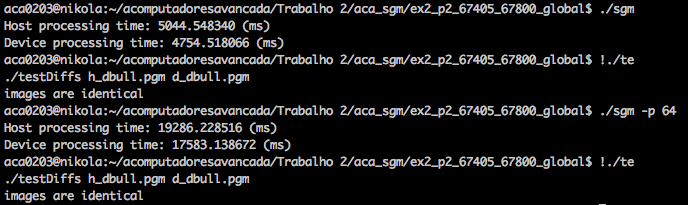
\includegraphics[width=100mm,scale=1]{IteratePositionsV1.png}
 \caption{\\ Resultados obtidos utilizando a versão 1 com global memory}
 \label{fig:IteratePositionsV1}
\end{figure}

Notaram-se algumas melhorias, contudo é possível melhorar o speedup, e para isso recorreu-se a uma segunda versão, desenvolvida com o apoio da leitura do artigo  \footnote{\label{url1} \href{http://elearning.ua.pt/mod/resource/view.php?id=217488}{Real-time Stereo Vision: Optimizing Semi-Global Matching, Matthias Michael, Jan Salmen, Johannes Stallkamp, and Marc Schlipsing, IEEE Intelligent Vehicles Symposium pp 1197-1202, 2013 }} fornecido pelos professores.

\newpage
\subsubsection{Global Memory - Versão 2}

Nesta segunda versão, decidiu-se alterar a geometria do kernel, de forma a que agora cada thread fosse responsável por um único valor de disparidade num path. Para isso a geometria criada para x foi a seguinte:

\begin{figure}[!htb]
\center
 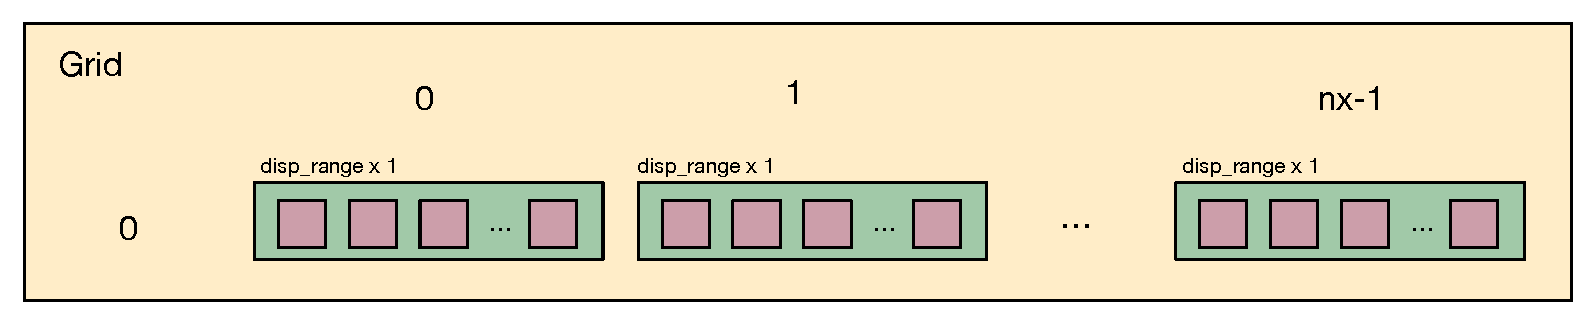
\includegraphics[width=50mm,height=100mm,scale=1]{IteratePositionDirxposneg_v2_kernel.pdf}
 \caption{\\ Geometria do Kernel para as funções iterate\_direction\_dirxpos() e iterate\_direction\_dirxneg()}
 \label{fig:IteratePositionDirxposneg_v2_kernel}
\end{figure}

A grid passa a ser composta por ny blocos, cada um com um número de threads igual ao \textit{disparity range}. Passa então a existir um bloco para cada linha em x, composto por threads, onde cada uma corresponde a um valor de disparidade diferente.

A implementação destes dois kernels foi efetuada através do seguinte algoritmo:

 \begin{lstlisting}[language=c++, basicstyle=\scriptsize]
__global__ void iterate_direction_dirxpos_dev(const int dirx, const int *left_image,
                        const int* costs, int *accumulated_costs,
                        const int nx, const int ny, const int disp_range ){

      int i = threadIdx.x;
      int j = blockIdx.y * blockDim.y + threadIdx.y;
      if(i < disp_range && j<ny){
        ACCUMULATED_COSTS(0,j,i) += COSTS(0,j,i);

      __syncthreads();


      for(int l = 1; l<nx;l++){
        evaluate_path_dev( &ACCUMULATED_COSTS(l-dirx,j,0),
                         &COSTS(l,j,0),
                         abs(LEFT_IMAGE(l,j)-LEFT_IMAGE(l-dirx,j)) ,
                         &ACCUMULATED_COSTS(l,j,0), nx, ny, disp_range, i);
        __syncthreads();

      }
    }
}

__global__ void iterate_direction_dirxneg_dev(const int dirx, const int *left_image,
                        const int* costs, int *accumulated_costs,
                        const int nx, const int ny, const int disp_range )
{
      int i = threadIdx.x;
      int j = blockIdx.y * blockDim.y + threadIdx.y;

      if(i < disp_range && j < ny){

        ACCUMULATED_COSTS(nx-1,j,i) += COSTS(nx-1,j,i);

        __syncthreads();


        for(int l = nx-2; l >= 0; l--){
            evaluate_path_dev( &ACCUMULATED_COSTS(l-dirx,j,0),
                           &COSTS(l,j,0),
                           abs(LEFT_IMAGE(l,j)-LEFT_IMAGE(l-dirx,j)),
                           &ACCUMULATED_COSTS(l,j,0), nx, ny, disp_range, i);
            __syncthreads();
        }
      }
}
\end{lstlisting} 

\newpage
No caso da direção ser em y, a geometria utilizada foi a seguinte:

\begin{figure}[!htb]
\center
 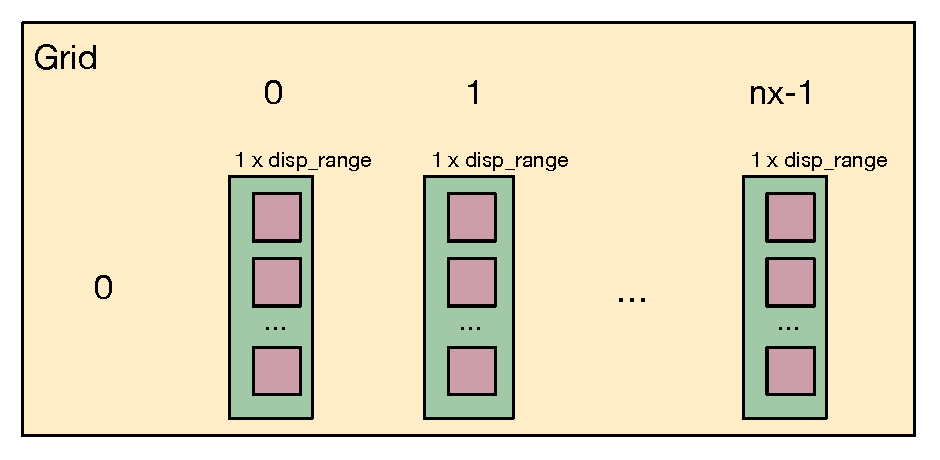
\includegraphics[width=100mm,scale=1]{IteratePositionDiryposneg_v2_kernel.pdf}
 \caption{\\ Geometria do Kernel para as funções iterate\_direction\_dirypos() e iterate\_direction\_diryneg()}
 \label{fig:IteratePositionDiryposneg_v2_kernel}
\end{figure}

Nesta situação, a grid é composta por nx blocos, cada um um número de threads igual ao disparity range, onde cada thread, tal como em x, é responsável por um valor de disparidade diferente.

A implementação dos kernels correspondestes a esta geometria é a seguinte:

 \begin{lstlisting}[language=c++, basicstyle=\scriptsize]
__global__ void iterate_direction_dirypos_dev(const int diry, const int *left_image,
                        const int* costs, int *accumulated_costs,
                        const int nx, const int ny, const int disp_range )
{
    int i = blockIdx.x * blockDim.x + threadIdx.x;
    int j = threadIdx.y;
    if(j < disp_range && i < nx){

        ACCUMULATED_COSTS(i,0,j) += COSTS(i,0,j);
        __syncthreads();

        for(int l = 1; l<ny; l++){

          evaluate_path_dev( &ACCUMULATED_COSTS(i,l-diry,0),
                         &COSTS(i,l,0),
                         abs(LEFT_IMAGE(i,l)-LEFT_IMAGE(i,l-diry)),
                         &ACCUMULATED_COSTS(i,l,0), nx, ny, disp_range, j);
          __syncthreads();

      }
    }
}

__global__ void iterate_direction_diryneg_dev(const int diry, const int *left_image,
                        const int* costs, int *accumulated_costs,
                        const int nx, const int ny, const int disp_range )
{

      int i = blockIdx.x * blockDim.x + threadIdx.x;
      int j = threadIdx.y;
      if(j < disp_range && i < nx){

        ACCUMULATED_COSTS(i,ny-1,j) += COSTS(i,ny-1,j);
        __syncthreads();


        for(int l = ny-2; l >= 0; l--){

            evaluate_path_dev( &ACCUMULATED_COSTS(i,l-diry,0),
                       &COSTS(i,l,0),
                       abs(LEFT_IMAGE(i,l)-LEFT_IMAGE(i,l-diry)),
                       &ACCUMULATED_COSTS(i,l,0) , nx, ny, disp_range, j);
            __syncthreads();

         }
      }
}

\end{lstlisting} 

Para que a implementação desta segunda versão funcionasse foi necessário recorrer ao comando \textit{\_\_syncthreads()}, de forma a que todas as threads esperassem umas pelas outras quando chegavam ao ponto onde este comando se encontra colocado, garantindo assim que tudo era feito sequencialmente, e posteriormente utilizado de maneira correta quando se recorresse à shared memory. Foi ainda necessário efetuar alterações no código da função \textit{evaluate\_path()} para que agora dentro deste apenas calculasse o valor necessário para aquele valor de disparidade, ficando assim:

  \begin{lstlisting}[language=c++, basicstyle=\scriptsize]
__device__ void evaluate_path_dev(const int *prior, const int *local,
                     int path_intensity_gradient, int *curr_cost ,
                     const int nx, const int ny, const int disp_range, const int d)
  {
    memcpy(curr_cost, local, sizeof(int)*disp_range);
    
    int e_smooth = NPP_MAX_16U;
    
    for ( int d_p = 0; d_p < disp_range; d_p++ ) {
      if ( d_p - d == 0 ) {
        // No penality
        e_smooth = MMIN(e_smooth,prior[d_p]);
        
      } else if ( abs(d_p - d) == 1 ) {
        // Small penality
        e_smooth = MMIN(e_smooth,prior[d_p]+PENALTY1);
        
      } else {
        // Large penality
        e_smooth =
          MMIN(e_smooth,prior[d_p] +
                   MMAX(PENALTY1,
                   path_intensity_gradient ? PENALTY2/path_intensity_gradient : PENALTY2));
      }
    }

    curr_cost[d] += e_smooth;

    int min = NPP_MAX_16U;
    
    for ( int d_s = 0; d_s < disp_range; d_s++ ) {
      if (prior[d_s]<min) min=prior[d_s];
    }
    
    curr_cost[d]-=min;
}

\end{lstlisting} 

Com esta nova implementação, a melhoria no speedup foi brutal, melhorando bastante os resultados:

\begin{figure}[!htb]
\center
 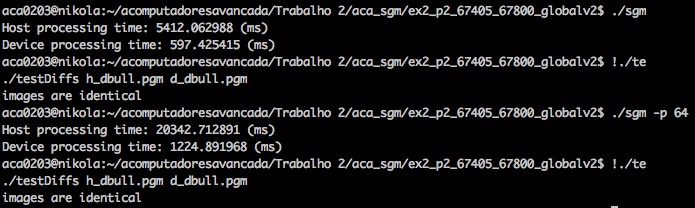
\includegraphics[width=100mm,scale=1]{IteratePositionsV2.png}
 \caption{\\ Resultados obtidos utilizando a versão 2 com global memory}
 \label{fig:IteratePositionsV2}
\end{figure}

Para melhorar ainda mais estes resultados passou-se a utilizar a \textit{shared memory} para o cálculo do path.

\newpage
\subsubsection{Shared Memory}

Visto que as threads na versão 2 eram executadas em paralelo, e que existiam valores que todas partilhavam e necessitavam umas das outras para o cálculo dos mínimos, então decidiu-se que seria mais produtivo que as pesquisas fossem feitas na \textit{shared memory}. Para isso, foi necessário criar um array de \textit{shared memory} com shared memory size igual a disparity\_range*sizeof(int), onde cada índice do array corresponde a um valor de disparidade.

A maioria das alterações foi feita na função \textit{evaluate\_path()}, visto ser nesta que se efetuam todas as pesquisas necessárias para determinar o current cost e o minimo. Com isto a função ficou da seguinte forma:

  \begin{lstlisting}[language=c++, basicstyle=\scriptsize]
__device__ void evaluate_path_dev(const int *prior, const int *local,
                     int path_intensity_gradient, int *curr_cost ,
                     const int nx, const int ny, const int disp_range, const int d, int shmem[])
  {
    memcpy(curr_cost, local, sizeof(int)*disp_range);
    
    int e_smooth = NPP_MAX_16U;

    for ( int d_p = 0; d_p < disp_range; d_p++ ) {
      if ( d_p - d == 0 ) {
        // No penality
        e_smooth = MMIN(e_smooth,shmem[d_p]);
        
      } else if ( abs(d_p - d) == 1 ) {
        // Small penality
        e_smooth = MMIN(e_smooth,shmem[d_p]+PENALTY1);
        
      } else {
        // Large penality
        e_smooth =
          MMIN(e_smooth,shmem[d_p] +
                   MMAX(PENALTY1,
                   path_intensity_gradient ? PENALTY2/path_intensity_gradient : PENALTY2));
      }
    }

    curr_cost[d] += e_smooth;

    int min = NPP_MAX_16U;
    
    for ( int d_s = 0; d_s < disp_range; d_s++ ) {
      if (shmem[d_s]<min) min=shmem[d_s];
    }
    
    curr_cost[d]-=min;
    
    __syncthreads();
    
    shmem[d] = curr_cost[d];

}

\end{lstlisting} 

Aqui foi também necessário colocar outra vez o comando \textit{\_\_syncthreads()}, para que todas as threads apenas escrevessem na memória partilhada quando todas tivessem calculado o mínimo valor nesta.

Mais uma vez com esta nova implementação, os resultados voltaram a melhorar muito em relação à memória global:

\begin{figure}[!htb]
\center
 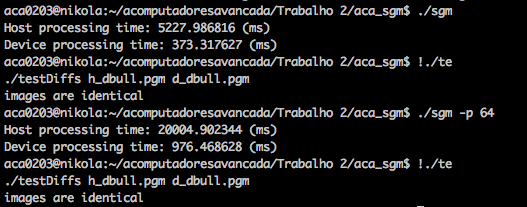
\includegraphics[width=100mm,scale=1]{IteratePositionShared.png}
 \caption{\\ Resultados obtidos utilizando shared memory}
 \label{fig:IteratePositionShared}
\end{figure}

\newpage
\section{Exercício 3}

\subsection{Cuda Kernel da função "inplace\_sum\_views()"}

A função \textit{inplace\_sum\_views}, tem como objectivo a soma de pixeis de duas imagens. Para esta a geometria utilizada foi idêntica à da determinação de custos (Exercício 1), contudo possui uma pequena alteração, pois o número de colunas é agora correspondente a ceil((nx*disp_range)/32):

\begin{figure}[!htb]
\center
 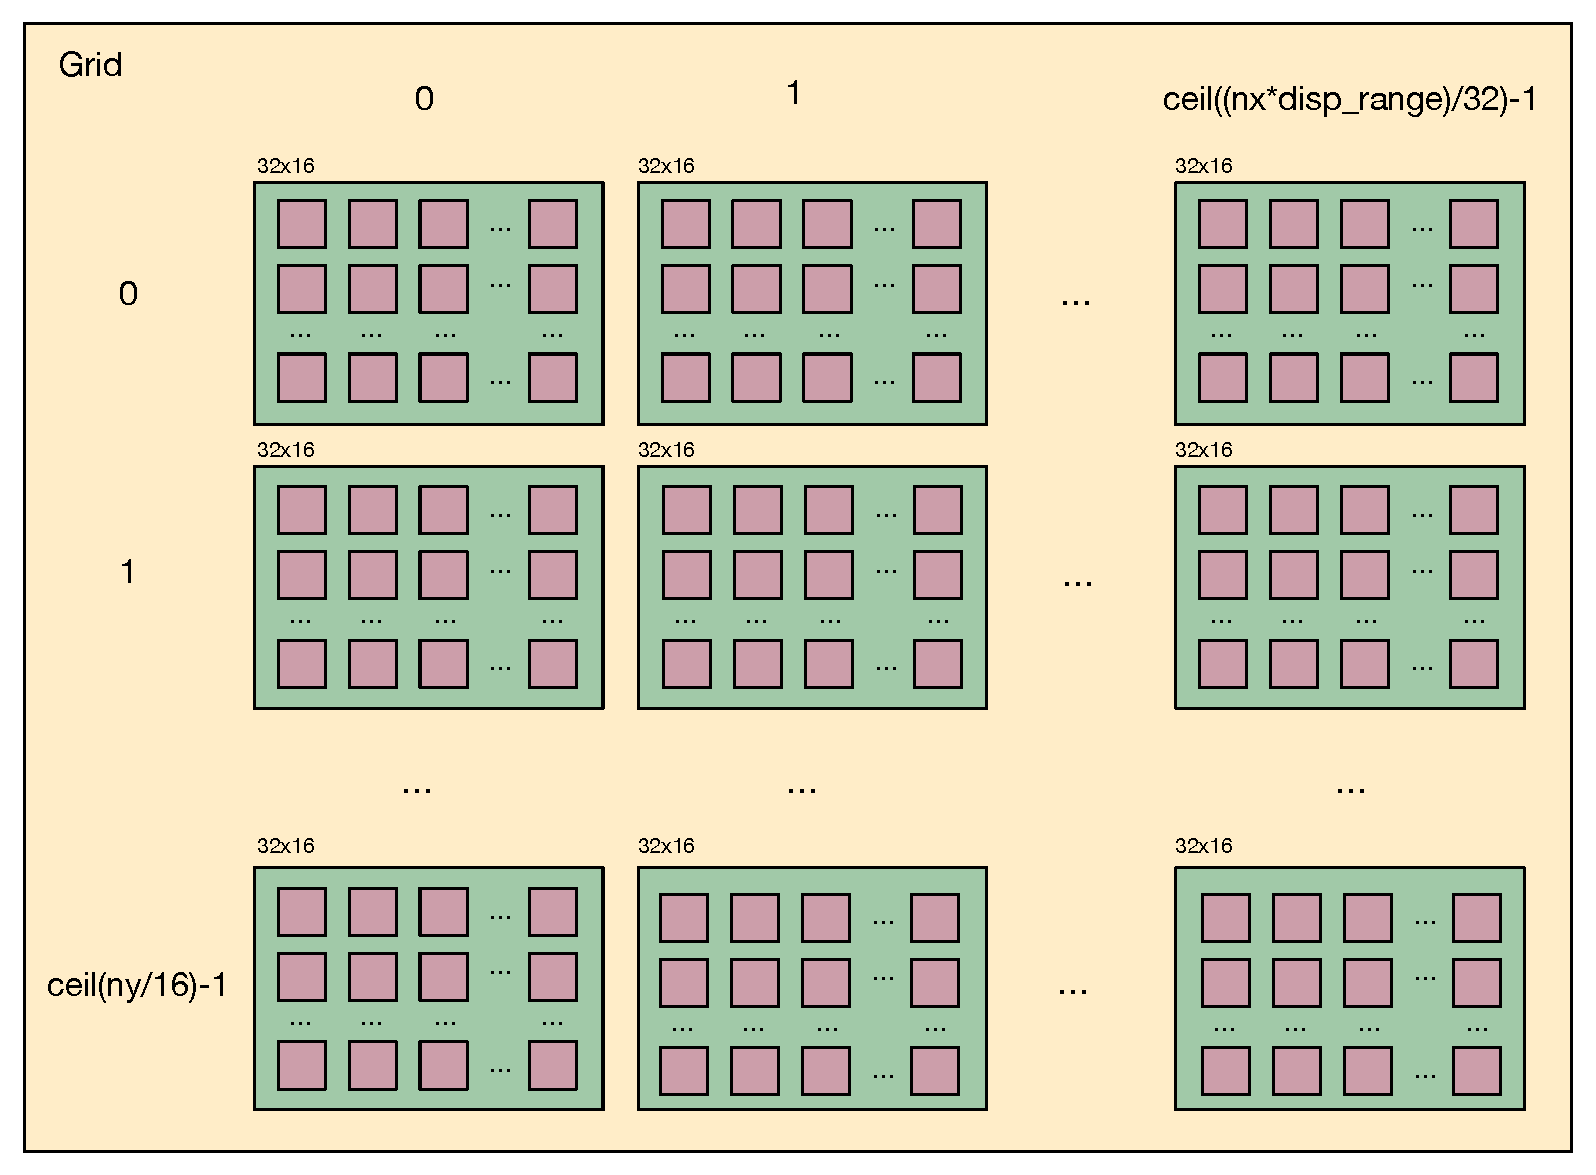
\includegraphics[width=100mm,scale=1]{InplaceSumViews_v1_kernel.pdf}
 \caption{\\ Geometria do Kernel para a função inplace\_sum\_views()}
 \label{fig:InplaceSumViews_v1_kernel}
\end{figure}

Para a implementação deste kernel criou-se o seguinte algoritmo:

  \begin{lstlisting}[language=c++, basicstyle=\scriptsize]
__global__ void inplace_sum_views_dev(int * im1, const int * im2,
                                      const int nx, const int ny, const int disp_range){
    
      int i = blockIdx.x * blockDim.x + threadIdx.x;
      int j = blockIdx.y * blockDim.y + threadIdx.y;
      int id = i + (j * (nx*disp_range));
      
      if(i < nx*disp_range && j < ny){
        int *im1_init = im1;
        im1 += id;
        im2 += id;
        if(im1 != (im1_init + (nx*ny*disp_range))  ){
          *im1 += *im2;
        }
      }
}

\end{lstlisting} 

Posteriormente a esta implementação obtiveram-se os seguintes resultados com a utilização do exercício 2 em memória global e em memória partilhada:

 

\newpage
\section{Conclusão}

Este trabalho foi útil para assentar todos os conhecimentos que se foi obtendo ao longo destes anos, tanto em Arquitectura de Computadores Avançada como em Arquitetura de Computadores I e II. Ambas as entregas foram primeiro planeadas em papel antes de se avançar para a implementação o que resultou em bons resultados a nível de tempo despendido, para ambos as entregas fez-se uso de dois dias de trabalho.

Na primeira entrega houve uma falha na implementação, esqueceu-se de realizar o shift left 2 do program counter para calcular o endereço para onde é suposto saltar a instrução jump.

Já na segunda entrega teve-se os máximos cuidados para que tudo funcionasse perfeitamente.

\end{document}